\chapter{Physics objects definitions} % Main chapter title

\label{Chapter5} % Change X to a consecutive number; for referencing this chapter elsewhere, use \ref{ChapterX}

\lhead{Chapter 5. \emph{Physics object definitions}} % Change X to a consecutive number; this is for the header on each page - perhaps a shortened title

CMS detector is designed in order to efficiently identify and reconstruct interesting physics objects. The reconstruction procedure which takes as input the signals from all the subdetectors and combines them to get physics objects is called \textit{particle flow}. \cite{CMS:2009nxa} This algorithm classifies all the objects into one of the following categories: charged hadrons, neutral hadrons, photons, electrons and muons. These are built from reconstructed tracks, energy deposits in the calorimeters and signals in the muon chambers creating a global event description. Additionally, a set of cuts is imposed on both input signals and reconstructed object in order to minimize the misidentification, e.g wrongly identifying electron as a jet. 
\par Following sections show electron and muon reconstruction procedures and identification criteria. Additionally, jet reconstruction procedure is described together with necessary jet corrections and b-tagging algorithms. After the reconstruction of all other objects, missing transverse energy is computed.

%----------------------------------------------------------------------------------------
%	SECTION 1
%----------------------------------------------------------------------------------------

\section{Electrons}

Electrons in CMS are detected as a track in tracking system and an energy deposit in the electromagnetic calorimeter. Two different algorithms are used for electron reconstruction, \textit{tracker driven} seeding which is more suitable for low $p_T$ electrons and electrons inside jets. O the other hand, \textit{ECAL driven} seeding is optimized for high $p_T$ isolated electrons. Both approaches take electromagnetic crystals with deposited energy and join them into \textit{clusters}. Electron passing through the detector bends due to magnetic field and interacts with the detector material emitting \textit{bremsstrahlung} photons. ECAL energy deposits from these photons are spread in $\phi$ direction in very narrow $\eta$ range and combined with the existing cluster forming a \textit{supercluster}. Trajectories are reconstructed using modeling of electron energy loss in detector material and fitted with a Gaussian Sum Filter(GSF)\cite{2005JPhG31N9A}.
\par Matching ECAL superclusters and reconstructed tracks is where the two approaches differ. Tracker driven seeding uses track from the electromagnetic calorimeter and tries to match it with the supercluster in the ECAL while ECAL driven seeding starts from the superclusters.
Each electron candidate has to pass various quality cuts in order to maximize the probability of identifying the electron coming from the hard interaction, and reject electrons from jets or conversion. These selection cuts can be divided into three categories: identification, isolation and conversion cuts. Details on electron reconstruction and performance can be found in \cite{CMS:2010bta}.

%-----------------------------------
%	SUBSECTION 1.1
%-----------------------------------
\subsection{Electron identification}
\label{sec:eleID}

Electron identification procedure first focuses on good matching between reconstructed track and supercluster, by imposing cuts on angular distance $\Delta \eta$ and $\Delta \phi$ between the two. These variables are computed as absolute $\eta$ and $\phi$ distance between the supercluster and electron track extrapolated to the ECAL surface. Additionally, a cut is imposed on $\sigma_{i\eta i\eta}$ which describes a shower shape spread in $\eta$ direction. This variable is particularly discriminating against clusters coming from electrons and energy deposits from photons and fakes. Shower shape is defined as:
\begin{equation}
\sigma_{i\eta i\eta} = \sqrt{\frac{\sum_{i}^{5\times 5} w_i(\eta_i-\eta_{seed})^2\times \Delta \eta^2_{xtal} }{\sum_{i}^{5\times 5}}}
\end{equation}
where $i$ is running over all crystals in $5\times5$ block around supercluster seed, $\eta_i-\eta_{seed}$ is the distance in number of crystals in $\eta$ direction between $i$-th crystal in supercluster and seed crystal and $\Delta \eta^2_{xtal}$ is the average width of a single crystal. Each crystal is given a weight defined as $w_i=max(0,4.7+ln(E_i/E_{5\times5}))$, where $E_i$ is a single crystal energy, and $E_{5\times 5}$ is the sum of energy deposits inside a 5$\times$5 crystal block. 
The ratio between the energy deposits in the hadronic calorimeter and electromagnetic calorimeter for electrons is used to discard the events with significant hadron activity.
\par Electrons coming from converted photons are rejected by requiring a hit in every layer of the inner tracking system. Additionally, for each electron track a fit is performed trying to combine it with another electron track under the hypothesis that both electrons originated from converted photon. Electron is selected only if this probability is sufficiently small. Electron compatibility with the primary vertex is estimated by looking at the impact parameters in both $xy$ and $z$ planes. Due to the gap in the electromagnetic calorimeter in 1.4442 $< |\eta| <$ 1.566, all electrons which have a supercluster position reconstructed in this range are rejected. A full list of identification criteria is summarized in Table \ref{tab:eleID}.
 \begin{table}[h]
\centering
  \caption{A summary of electron identification criteria.}
  \label{tab:eleID}
  \begin{tabular}{ l  c c}
      \hline
      \hline
      	Variable & Barrel & Endcap \\
      	\hline
    		$\Delta\eta$ $<$ &  0.004 & 0.005 \\
     	$\Delta\phi$ $<$ &  0.03 & 0.02 \\
     	$\sigma_{i\eta i\eta}$ $<$ & 0.01 & 0.03 \\
		$H/E$ $<$ & 0.12 & 0.10 \\
		$d_{xy}$ $<$ & 0.02 cm & 0.02 cm \\
		$d_{z}$ $<$  & 0.1 cm & 0.1 cm \\
		$(1/E - 1/p)$ $<$ & 0.05 & 0.05\\
		Missing hits  & 0 & 1 \\
		Vertex Fit Probability & $10^{-6}$ & $10^{-6}$ \\    	

      \hline
      \hline 
  \end{tabular}
\end{table}


%----------------------------------------------------------------------------------------
%	SECTION 2
%----------------------------------------------------------------------------------------

\section{Muons}

Muons in CMS are reconstructed by combining a reconstructed track inside the tracker(\textit{tracker track}) and track in muon chambers (\textit{standalone muon track}). Individual track segments in the muon chambers are fitted using Kalman fitter technique \cite{Fruhwirth1987444}  in order to obtain a standalone muon track. Similar as with electrons, two approaches are used for combining tracker track and standalone track. \textit{Global muon reconstruction} approach uses a standalone muon track in the muon chambers and tries to find a matching tracker track by combining parameters of two tracks by projecting it to the common surface. This \textit{outside-in} approach uses Kalman fitter technique to combine these two objects in an object called \textit{global muon}. Muon momentum is then determined from this global muon track using all available systems which shows improved precision in comparison to other approaches.  
\par The second approach for muon reconstruction is \textit{tracker muon reconstruction} which starts from tracks inside the tracker with $p_T>0.5$ GeV/c and total momentum $p>2.5$ GeV/c as potential muon candidates. Extrapolation is than performed to the muon chambers taking into account the magnetic field, Coulomb scattering in the material and other energy losses. \textit{Tracker moun} is found if at least one muon segment matches the extrapolated track. The efficiency of the \textit{Tracker muon} reconstruction is higher for low energy muons than the efficiency for the global muons, because only a single muon segment in the muon chambers is required. For high energy muons where more there are more segments inside muon chambers, \textit{global muon} algorithm is designed to have high efficiency.    

%-----------------------------------
%	SUBSECTION 2.1
%-----------------------------------

\subsection{Muon identification}
\label{sec:muID}

In this analysis \textit{particle flow} muon identification selection is applied to the \textit{global muons}. Selection is applied in order to minimize misidentification of charged hadrons as muons, maximize the efficiency of identification of muons inside jets and ensure good momentum measurement. Muons used in the analysis have $|\eta|<2.1$ and transverse momentum $p_T<30$ GeV with more than 5 hits in the inner tracker system and at least one hit in pixel detector. At least one good muon chamber hit in the \textit{global muon} track fit is required to have $\chi^2/ndof<10$, at least two segments in two different muon stations should be matched to a track in order to suppress muons from in-flight decays. Cosmic muons are rejected by applying cuts on the impact parameter with respect to the primary vertex of $|d_{xy}|<$0.2 cm and $|d_z|<$ 0.5 cm. Muon identification criteria is summarized in Table \ref{tab:muID}.

  \begin{table}[h]
\centering
  \caption{A summary of muon identification criteria.}
  \label{tab:muID}
  \begin{tabular}{ l  c c}
      \hline
      \hline
      	Variable & Requirement \\
      	\hline
    		number of pixel hits $>$ &  0 \\
     	number of inner tracker hits $>$ &  5 \\
     	$\chi^2/ndof$ $<$ & 10 \\
		number of muon hits $>$ & 0  \\
		chambers with matched segments $>$ & 1  \\		
		$d_{xy}$ $<$ & 0.2 cm \\
		$d_{z}$ $<$  & 0.5 cm \\
      \hline
      \hline 
  \end{tabular}
\end{table}
 

%-----------------------------------
%	SUBSECTION 2.2
%-----------------------------------

\section{Lepton isolation}
Leptons from W decays are in general expected to be well isolated. The degree of isolation is calculated using \textit{particle flow} approach by summing the transverse momenta contributions of particles around the lepton inside a specific cone. All charged particles are considered as well as photons and neutral hadrons with $p_T>$0.5 GeV. The cone used for determination of energy deposits is defined as $\Delta R = \sqrt{\Delta \phi^2+ \Delta \eta^2}$ around the lepton axis and isolation measure is defined as:
\begin{equation}
I_{PF}^{rel} = \frac{\sum p_T^{charged} + max(0, \sum E_T^{\gamma}+\sum E_T^{neutral}-0.5\sum E_T^{PU})}{p_T^l}
\end{equation}
where $p_T^{charged}$ is the sum of the momenta of charged hadrons and $E_T^{\gamma} $ and $E_T^{neutral}$ are the sums of photon and neutral hadron momenta. $E_T^{PU}$ is the sum of the pile-up transverse energies from neutral particles and is calculated as a sum of track transverse momenta not coming from the primary vertex inside the isolation cone. This is divided by the factor of 0.5 which corresponds approximately to the ratio of neutral to charged hadron production in the hadronization process of pile-up interactions. Selected muons are required to pass isolation cut $I_{rel}^{PF}<0.12$ and in case of additional muon veto $I_{PF}^{rel}<0.2$. Electron isolation is computed in the same way with cut of $I_{rel}^{PF}<0.1$ for selected electrons and $I_{rel}^{PF}<0.15$ for vetoed additional electrons.


%----------------------------------------------------------------------------------------
%	SECTION 3
%----------------------------------------------------------------------------------------

\section{Jets}

In high energy physics, jet is a collimated group of hadrons which emerges as a result of quark or gluon fragmentation and hadronization process. Hadrons reconstructed in a particle detector need to be combined in order to form a jet and give information about the initial parton. A set of rules has to be created for how to group particles and how to assign momentum to the new jet. Usually this is done by summing the four-momentum of each particle in a jet.

%-----------------------------------
%	SUBSECTION 3.1
%-----------------------------------

\subsection{Jet algorithms}

Jet algorithms are taking into account the distance between particles and define rules which determine which particle belongs to which jet. Same jet algorithms should be applicable to both, experimental data and theoretical calculation.  Other important properties of jet algorithms is \textit{infrared safety} and \textit{collinear safety} which means is an event is modified by addition of soft emission of collinear splitting, the final number of hard jets will remain unchanged. These two properties together are called \textit{IRC safety}. IRC unsafe jet algorithms may break the cancellation of divergences by yielding one set of jets for tree-level splitting while loop diagrams lead to another, as shown if figure \ref{fig:jet_unsafe}, giving infinite cross-sections in the final calculations. Jet definitions, jet relation to partons and an overview of different jet algorithms are summarized in \cite{Salam:2009jx}.
\begin{figure}[htbp]
	\centering
		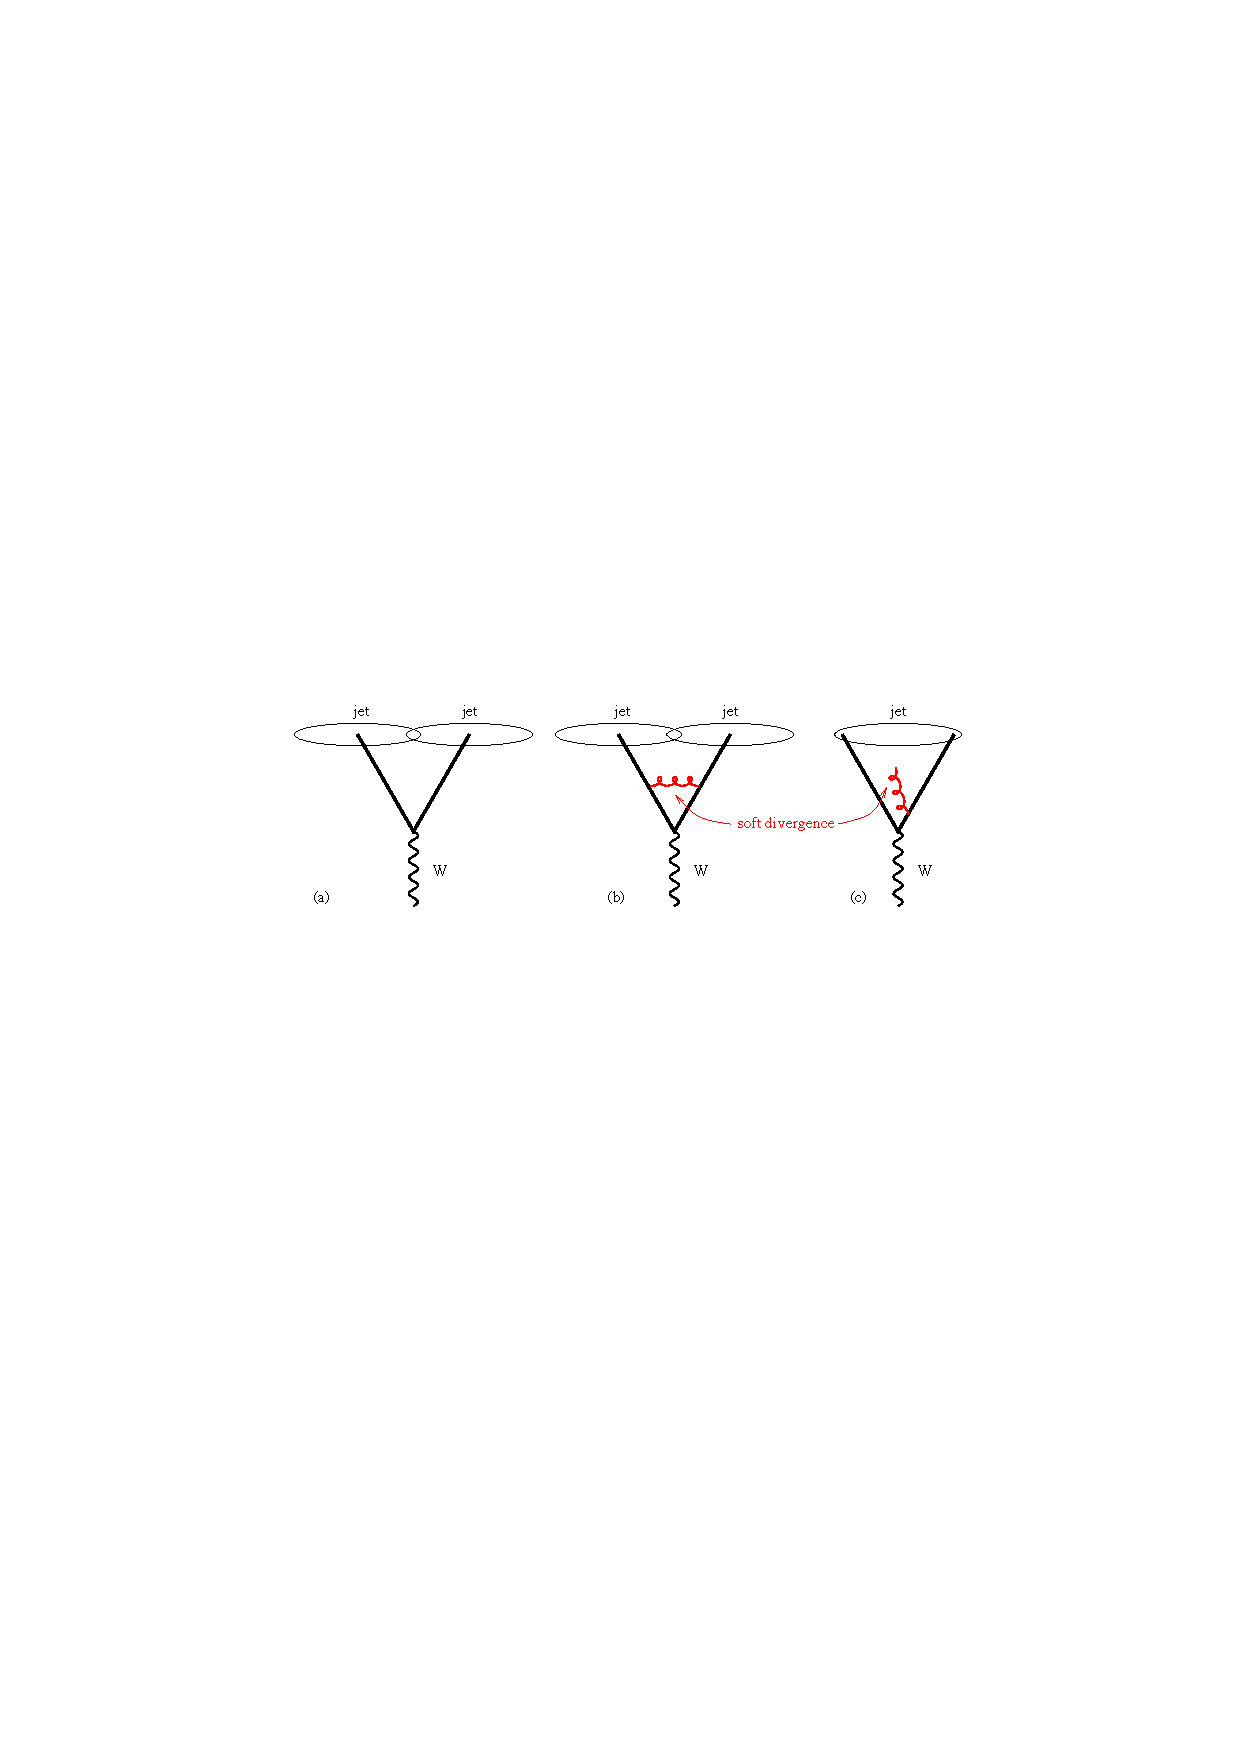
\includegraphics[width=0.8\textwidth]{Figures/jet_unsafe2.pdf}
		%\rule{35em}{0.5pt}
	\caption[An example of configuration of IRC unsafe jet algorithm.]{Configuration showing IC  unsafety with W boson and two partons. Adding a soft gluon causes two jets to be reconstructed as one. \cite{Salam:2009jx}}
	\label{fig:jet_unsafe}
\end{figure}

\par There are two types of jet algorithms which are most commonly used: \textit{cone algorithms} and \textit{sequential recombination algorithms}. In the case of \textit{cone algorithms}, a jet is defined as a set of particles inside a stable cone around their center of mass. Most popular cone algorithm is \textit{iterative cones} (IC) where a seed particle is chosen and momenta of all particles around that initial particle inside a cone of radius $R$ are summed. After adding each new particle to the sum, the direction of the new sum is taken as a seed direction, and the procedure repeats until the direction of the resulting cone is stable. Particles inside the cone are than removed from the list of available particles and the procedure repeats. This approach is not IRC safe as nearly collinear splitting of the hardest particle in the event can be reconstructed as two jets thus leaving another, less energetic, particle, pointing in another direction, to become the hardest particle in the event, yielding different set of jets. Cone algorithms can be IRC safe using a \textit{seedless cone} (SC) algorithm where all stable cone solutions are identified at once. However this approach is very time consuming even for small number of particles and thus very impractical to use.
In the \textit{sequential recombination algorithms} at hadron colliders two longitudinally invariant distances are introduced: $d_{ij}$ which is the distance between each pair of particles and $d_iB$ which is the particle-beam distance. These distances are defined as: 
\begin{equation}
d_{ij} = min(k_{T,i}^{2p},k_{T,j}^{2p}) \frac{\Delta R_{ij}^2}{R^2}
\end{equation}
\begin{equation}
d_{iB}=k_{T,i}^2p
\end{equation}
where $\Delta R_{ij}$ denotes the distance in the $\eta -\phi$ plane and is computed as $$\Delta R_{ij}^2 = (\eta_i-\eta_j)^2+(\phi_i-\phi_j)^2$$. $R$ is an angular cut-off, similar to the one in \textit{cone algorithms} and $p$ defines which particles are clustered first which is described below. Both are free parameters of the algorithm. The algorithm is applied using the following approach: first two distances $d_{ij}$ and $d_iB$ are computed and minimal values are found. If $d_{ij}$ is smaller, that two particles are combined, treated as a new particle and the distance with next particle in the list is computed. In case of $d_iB$ being smaller, $i$ is declared to be the final jet is removed from the list of particles. The procedure continues until there are no more particles in the list.
\begin{figure}[htbp]
	\centering
		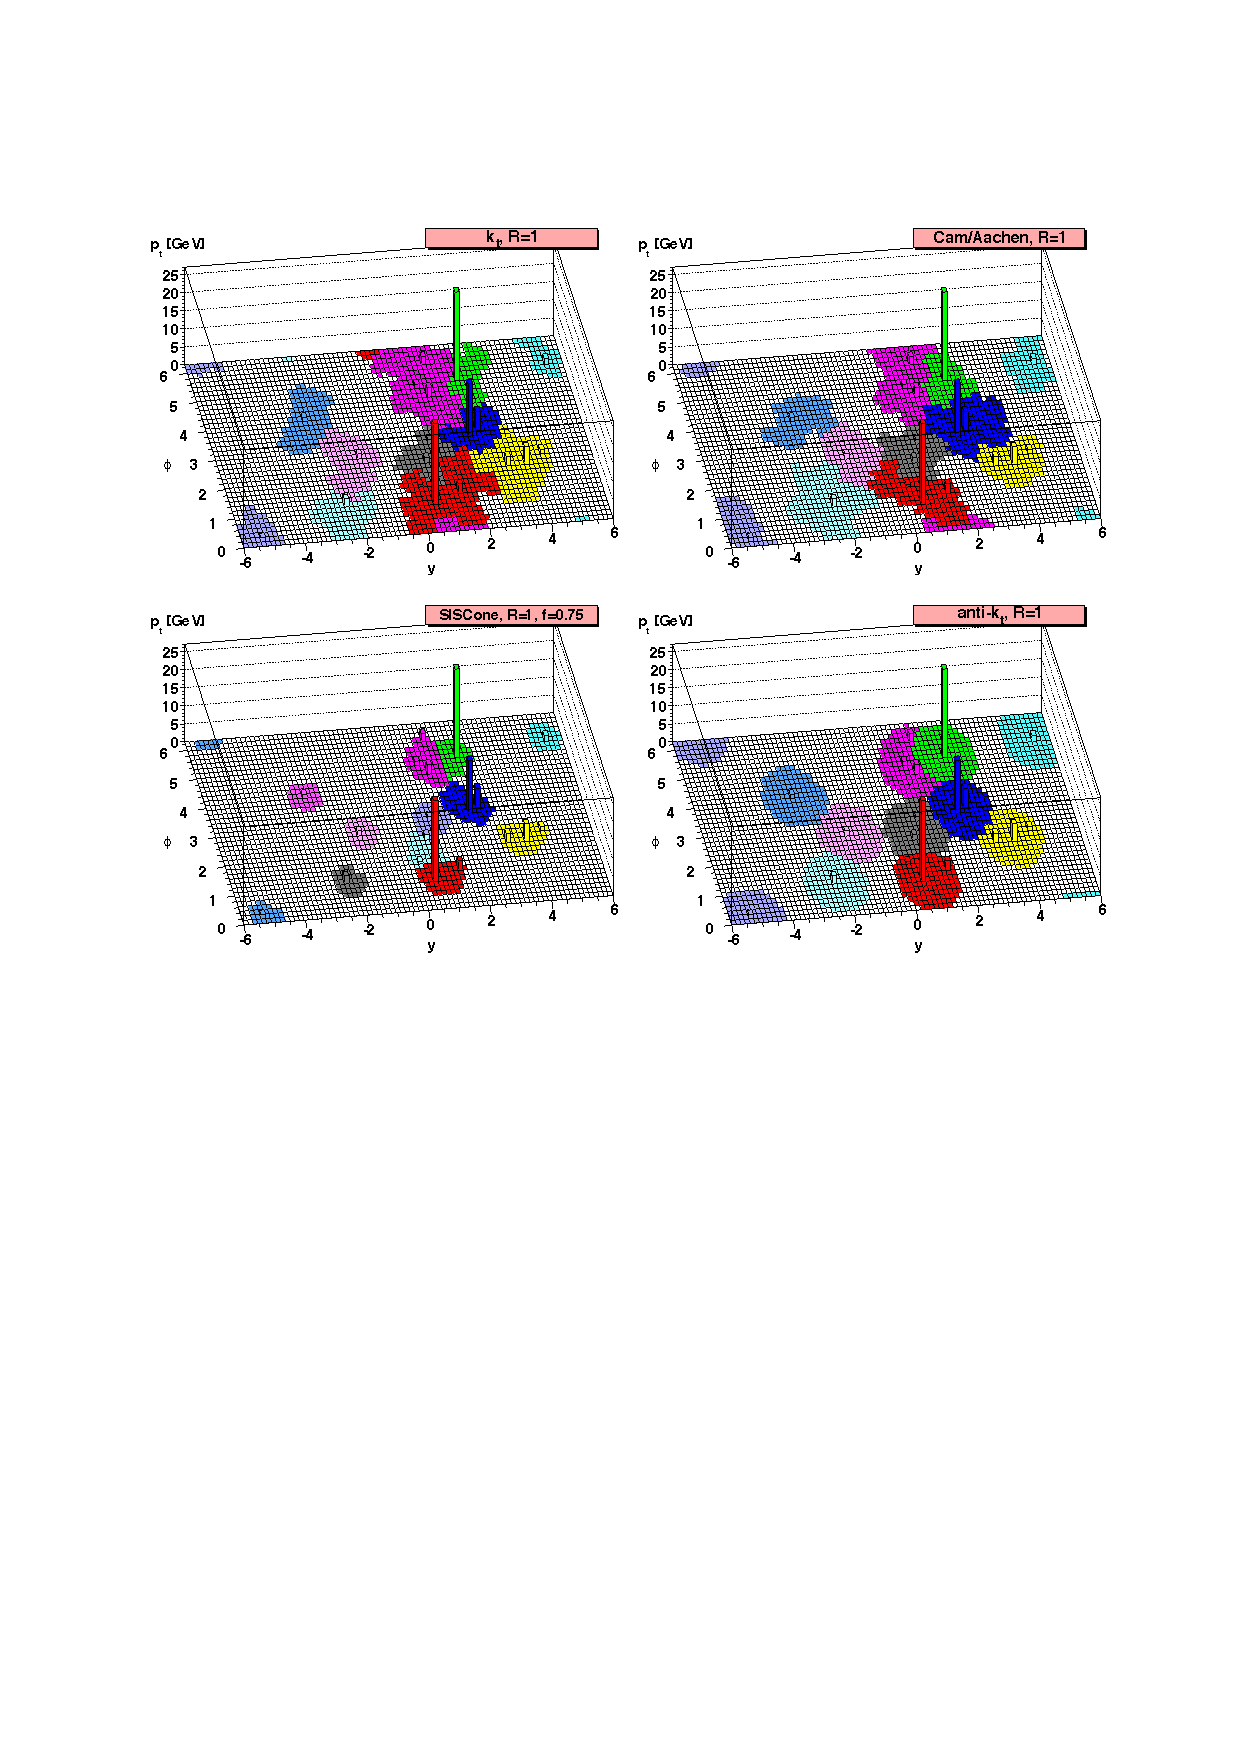
\includegraphics[width=0.9\textwidth]{Figures/diff_algos.pdf}
		%\rule{35em}{0.5pt}
	\caption[Clustering particles into jets with different algorithms.]{Clustering same set of reconstructed particles into jets using different jet algorithms. \cite{Salam:2009jx}}
	\label{fig:jetAlgos}
\end{figure}
\par Parameter $p$ defines which particles are clustered first thus defining the type of algorithm. The $k_T$ algorithm uses $p=1$, clustering soft particles first. This results in irregularly shaped jets, as shown in figure \ref{fig:jetAlgos}, which are sensitive to radiation in the event and difficult to calibrate. The \textit{Cambridge-Aachen} algorithm (CA) uses $p=0$ thus relying only on angular distribution of the input particles. This approach is particularly useful for jet substructure analysis and is less sensitive to radiation. The algorithm used in this analysis is $anti-k_T$ algorithm where $p=-1$ clusterizing the hardest particles first \cite{Cacciari:2008gp}. $Anti-k_T$ is an IRC safe algorithm with jets that are circular in shape because they are not affected by the softer components of the jet.       


%-----------------------------------
%	SUBSECTION 3.2
%-----------------------------------

\subsection{Jet corrections}
\label{sec:jetCorr}

Measured jet energy at detector level in general doesn't correspond to the energy of the originating particle. Jet calibration procedure is introduced to compensate for the nonlinear response of the calorimeters. This is done using a factorized approach where corrections on each level of correction are determined separately as described in \cite{Chatrchyan:2011ds}. Final corrected jet momentum is obtained from measured $p^{raw}$ according to:
\begin{equation}
p^{corr} = C_{offset}(p_T^{raw},\eta)\times C_{rel}(\eta) \times C_{abs}(p'_T) \times C_{res}(p_T'',\eta) \times p^{raw}
\end{equation}     
where offset correction $C_{offset}$ and calibration factors $C_{rel}$ and $C_{abs}$ are applied to both data and simulation, $C_{res}$ is applied only to data. Corrections are applied sequentially, in a fixed order such that $p_T' = C_{offset} \times C_{rel}(\eta) \times p^{raw}$ , and $p_T'' = C_{rel}(\eta) \times C_{abs}(p'_T)$. Correction factors used in this analysis can be found in \cite{CMS-DP-2013-033}.
Each level of corrections is summarized below:
\begin{itemize}
\item Offset correction $C_{offset}$ compensates for energy contributions arising from pile-up events or instrument noise. The offset is determined in dependence of pseudorapidity, jet area $p_T density$ which is described in \cite{Cacciari2008119}.
\item Relative correction $C_{rel}$ is aimed to flattening the jet scale in pseudorapidity. The correction is determined from simulation, adjusting the jet scale in all $\eta$ regions to one of the jets in $|\eta|<1.3$ without changing the absolute scale.
\item Absolute correction $C_{abs}$ flattens the jet scale in $p_T$. This correction is also determined from QCD multijet events as inverse of average response at fixed $p_T^{gen}$.
\item Residual correction $C_{res}$ is applied only to data in order to account for possible residual differences in data and simulation agreement after applying absolute and relative corrections. These corrections are derived using events with momentum balance in transverse plane, like dijet events or $Z/\gamma$ + jet events.
\end{itemize}
The total jet correction for a fixed jet $p_T$ as a function of pseudorapidity is shown in figure \ref{fig:tot_corr_eta}.
\begin{figure}[htbp]
	\centering
		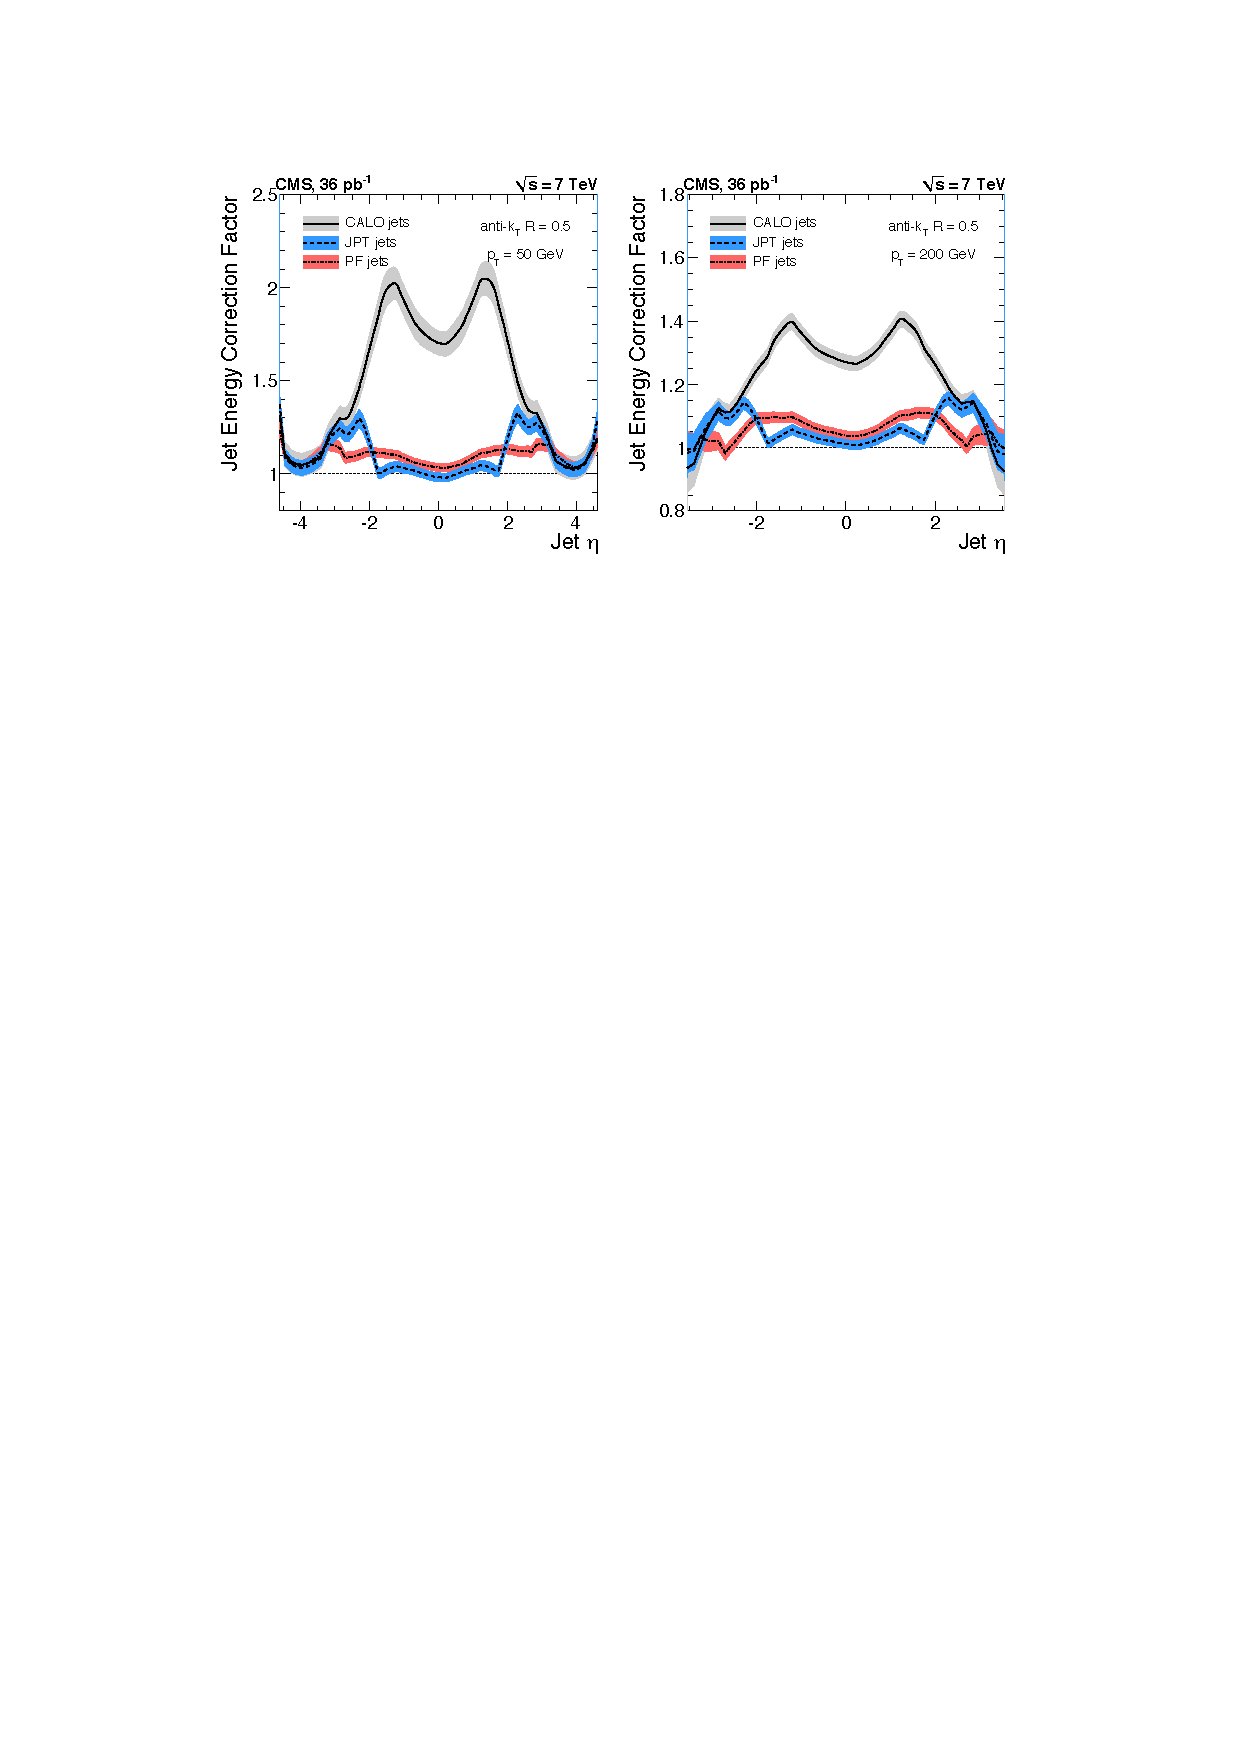
\includegraphics[width=0.9\textwidth]{Figures/jet_tot_corr_eta.pdf}
		%\rule{35em}{0.5pt}
	\caption[Total jet energy correction as a function of pseudorapidity of two different jet $p_T$ values.]{Total jet energy correction as a function of pseudorapidity of two different jet $p_T$ values. Corrections are shown for all three types of jets, calo, JPT and PF jets. Bands indicate corresponding uncertainty.}
	\label{fig:tot_corr_eta}
\end{figure}

\begin{figure}[htbp]
	\centering
		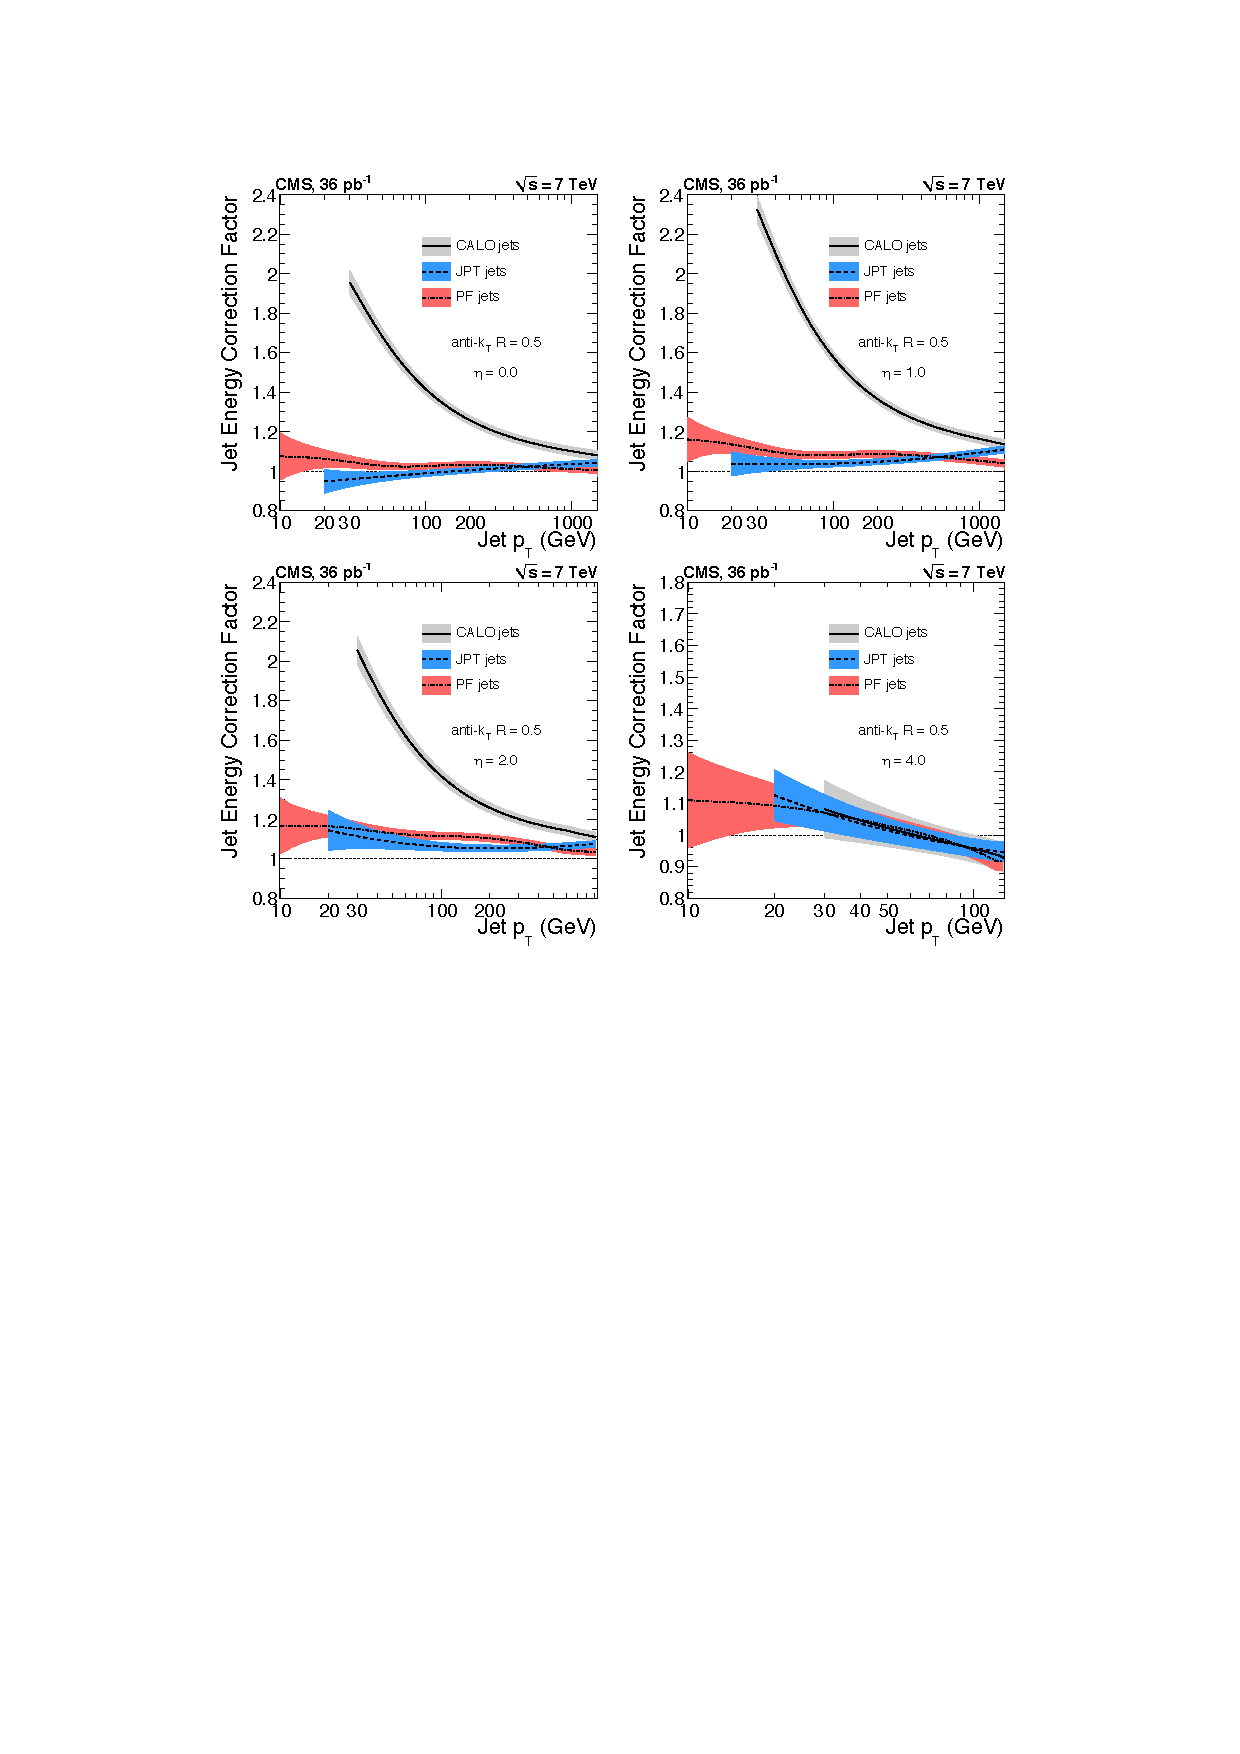
\includegraphics[width=0.9\textwidth]{Figures/jet_tot_corr_pt.pdf}
		%\rule{35em}{0.5pt}
	\caption[Total jet energy correction as a function of transverse momentum for four different $\eta$ values.]{Total jet energy correction as a function of transverse momentum for four different $\eta$ values. Corrections are shown for all three types of jets, calo, JPT and PF jets. Bands indicate corresponding uncertainty.}
	\label{fig:tot_corr_pt}
\end{figure}
%-----------------------------------
%	SUBSECTION 3.3
%-----------------------------------

\subsection{Jet identification}
\label{sec:jetID}
This analysis uses $anti-k_T$ algorithm with cone size $R=0.5$. Jet algorithm implementation is done in the \textit{Fast-jet} package \cite{Cacciari:2011ma}. Depending on which signals is the algorithm applied to, there are different kinds of jets: calo jets (using calorimeter deposits), jet-plus-track jets (calorimeter deposits complemented with tracker information) and most widely used \textit{particle flow} jets (PF). These jets are clustered from PF particles identified with PF algorithm, thus using the information not only from HCAL, but also from tracking system and ECAL which show much better resolution. Only neutral fraction of the jet is measured only with HCAL which makes about 15$\%$ of the total jet composition. PF jets show excellent performance and are the default jets for most CMS analysis. Pile-up information is also taken into account by removing charged hadrons originating from pile-up vertices from the list of particles available for the jet clusterization. This procedure is called \textit{charged hadron subtraction}. Some additional cuts to the jet composition are applied in order to endure good jet identification.  
  \begin{table}[h]
\centering
  \caption{A summary of jet identification criteria.}
  \label{tab:jetID}
  \begin{tabular}{ l  c c}
      \hline
      \hline
      	Variable & Requirement \\
      	\hline
    		Neutral hadron fraction & $<$ 0.99  \\
     	Neutral EM fraction & $<$ 0.99 \\
     	Number of Constituents & $>$ 1 \\		
		\hline
		Additional cuts for $|\eta|<2.4$ \\
		\hline
		Charged hadron fraction & $>$ 0 \\ 
		Charged multiplicity & $>$ 0 \\
		Charged EM fraction & $<$ 0.99 \\
      \hline
      \hline 
  \end{tabular}
\end{table}

%-----------------------------------
%	SUBSECTION 3.4
%-----------------------------------

\subsection{Jets from b quarks}
\label{sec:btagging}

Unique properties of the bottom quark can be used to identify hadronic jets originating from b quarks which are usually referred to as b-jets. Long lifetime of B hadrons is a consequence of weak force decay which results in their displacement by few micrometers at the LHC energies. B hadron decays show a large number of tracks with hard $p_T$ spectrum and soft leptons emerging from semi-leptonic decays. The process of b-jet identification is called $b-tagging$. This process takes one or more variables and produces a single discriminant value for each jet. This value shows how much the observed jet looks like a b-jet. There are several \textit{b-tagging} algorithms in use at CMS which are described in detail in \cite{Chatrchyan:2012jua} and the following were used in 2012 data analysis:
\begin{itemize}
	\item \textit{Track counting}(TC) - The discriminant value is the impact parameter significance which is calculated as impact parameter value divided by the respective impact parameter uncertainty. Impact parameter values are sorted in the decreasing order. Depending on whether second or third value is chosen, the algorithm is denoted as high efficiency or high purity. 
	\item \textit{Jet Probability}(JP) - This algorithm combines information from several tracks inside a jet by computing a likelihood thet all tracks originated from the primary vertex.  
	\item \textit{Combined secondary vertex}(CSV) - This is the most efficient \textit{b-tagging} algorithm currently used at CMS. Both secondary vertex and track related information are combined to build a CSV discriminant value. It shows high efficiency even when no good secondary vertex can be reconstructed. Some of the variables used in CSV algorithm are flight distance, vertex mass, impact parameter significance, track multiplicity at the vertex and track multiplicity in a jet. The distribution of CSV discriminant value is shown in figure \ref{fig:csv}.
\end{itemize}
\begin{figure}[ht]
	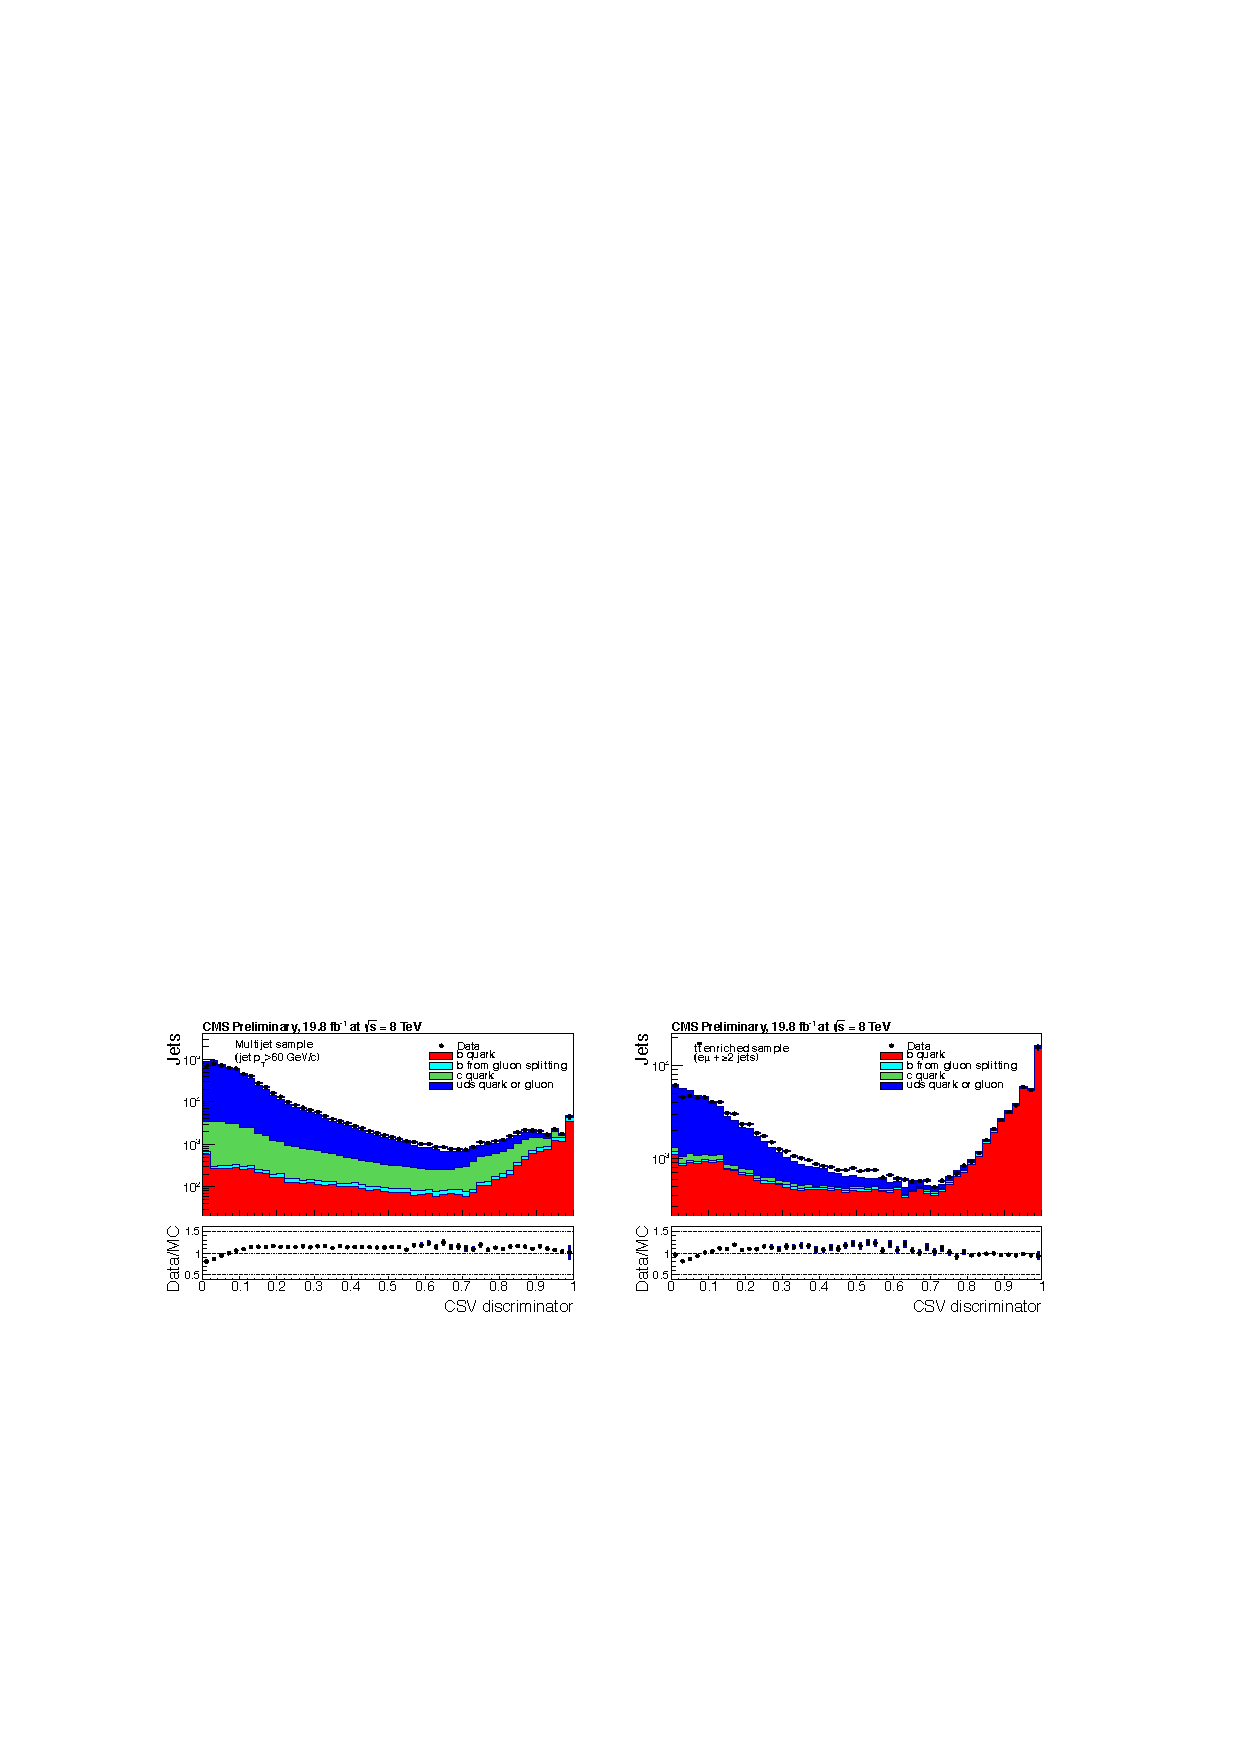
\includegraphics[width=\textwidth]{Figures/b-tag_csv.pdf}
	\caption{Combined secondary vertex discriminant value for multijet QCD sample (left) and tt enriched sample(right)\cite{CMS:2013vea}}
	\label{fig:csv}
\end{figure}
For each non-b-jet there is a chance that it would be identified as b-jet. Based on this misidentification rate, three operating points have been defined for the discriminant value: loose, medium and tight. For an average jet of 80 GeV, these values correspond to misidentification rates of 10\%, 1\% and 0.1\% respectively. Misidentification probabilities as a function of b-jer efficiency for several algorithms are shown in figure \ref{fig:misID}. 
\begin{figure}[ht]
\centering
	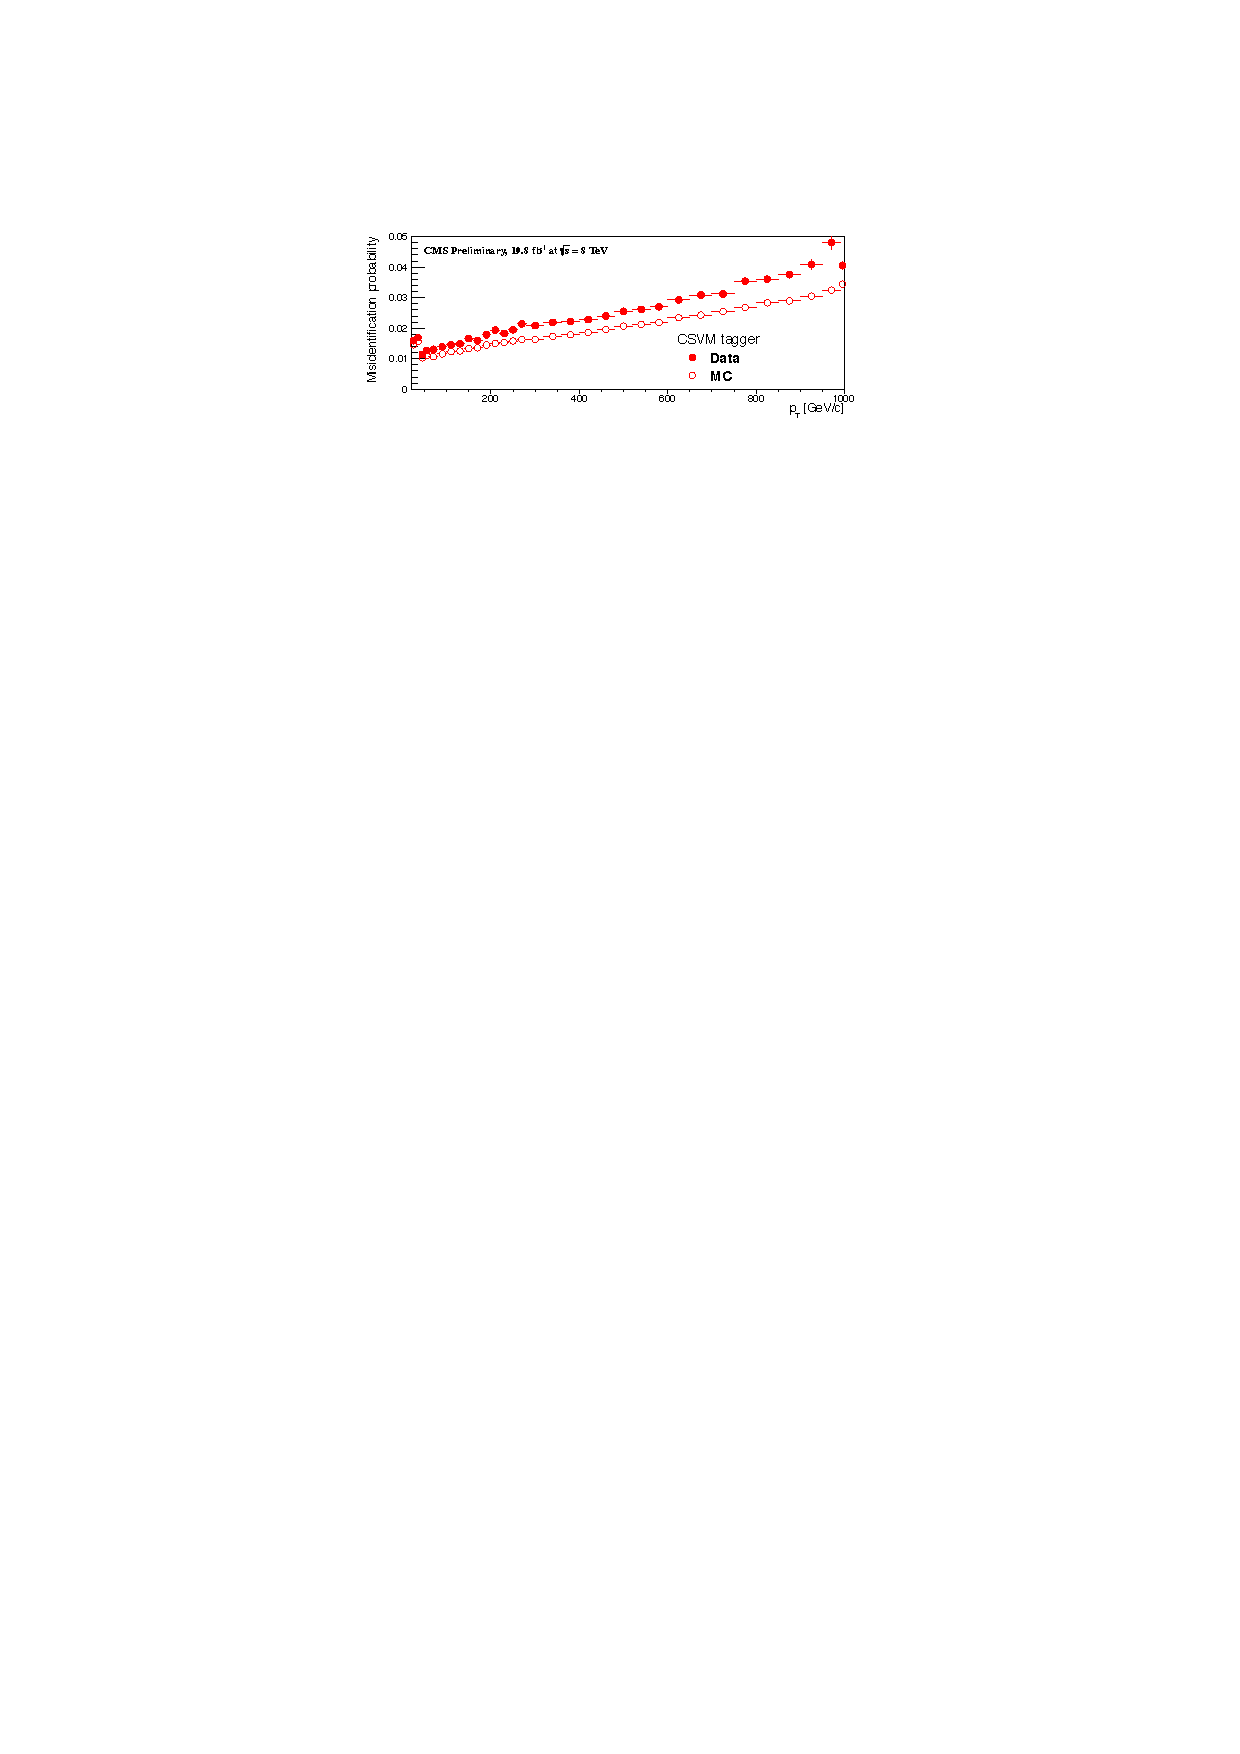
\includegraphics[width=0.6\textwidth]{Figures/MisID_CSVM.pdf}
	\caption{Combined secondary vertex misidentification probability for data and MC for medium working point.\cite{CMS:2013vea}}
	\label{fig:misID}
\end{figure}



%----------------------------------------------------------------------------------------
%	SECTION 4
%----------------------------------------------------------------------------------------

\section{Missing transverse energy}

Missing transverse momentum is the imbalance in the vectorial sum of transverse momenta of all measured particles. Momentum conservation delegates that the imbalance arises from weakly interacting neutral particles such as neutrinos. Missing transverse energy is the magnitude of the missing transverse momentum and is calculated as:
\begin{equation}
E_T^{miss}= |-\sum_{i} \vec{p}_i|
\end{equation}
where $i$ goes over all visible particles. Measurement of the missing transverse energy relies on the good measurement of all other particles in the event and as such is very sensitive to detector inefficiencies, particle missmeasurements, limited acceptance of the detector, cosmic-ray particles all of which can cause artificial missing energy. There are several approaches to determine $E_T^{miss}$. In this analysis, particle flow technique is used which tries to identify each particle in the event by combining the information from all subdetectors and gives the best missing energy resolution.\cite{CMS-PAS-PFT-09-001,Chatrchyan:2011tn} Several corrections are applied to the $E_T^{miss}$ which correct for the possible bias in the missing energy measurement:
\begin{itemize}
\item Type-I correction: propagates jet energy corrections described in Section \ref{sec:jetCorr} to missing energy. This correction replaces the missing energy calculated by summing transverse momenta of particles in a jet by transverse momentum of a jet to which JEC were applied.
\item xy-shift correction: aimed at correcting the observed missing energy $\phi$ modulation. True missing energy distribution is expected not to depend not to depend of $\phi$ because of the rotational symmetry of collisions around the beam axis. The possible cause for such modulation  include unisotropic detector response, detector misalignment, the displacement of the beam spot. The amplitude of the modulation is observed to increase with the number of pile-up interactions so this correction can be seen as mitigation for the pile-up effects.
\end{itemize}




